\documentclass[level=3]{kidscode}
%% Student "I can..." rubric: one row per statement, four tick boxes.
\newenvironment{icanrubric}{\par\noindent\renewcommand{\arraystretch}{1.5}%
  \tabularx{\linewidth}{@{}X*{4}{>{\centering\arraybackslash}p{1.75cm}}@{}}
  \toprule
  \rowcolor{kcaccent!15}\textbf{I can\ldots} & {\small\textbf{Just starting}} & {\small\textbf{Getting there}} & {\small\textbf{Got it}} & {\small\textbf{Expert}}\\ \midrule}
  {\bottomrule\endtabularx\par}
\newcommand{\ican}[1]{#1 & \Large$\square$ & \Large$\square$ & \Large$\square$ & \Large$\square$\\}
%% A numbered question heading: \question{Predict}{What does it print?}
%% Keep each code box on one page of the printed paper.
\tcbset{kccode/.append style={unbreakable}}
\newcounter{kcq}
\newcommand{\question}[2]{\par\needspace{5\baselineskip}\stepcounter{kcq}\medskip
  \noindent{\large\bfseries\color{kcaccent}Q\arabic{kcq}.\ #1}\par\nopagebreak\noindent #2\par}

\begin{document}
\kctitle{Assessments}{Placement quiz \textperiodcentered\ Mid-level checkpoint \textperiodcentered\ Exit assessment}

\begin{tip}[For students: read this first]
These papers are not tests you pass or fail. They show you (and your teacher) what you already
know and what to practise next. Write your answers on the paper. If you are stuck, write what you
\emph{think} and why --- that counts too. No computer needed unless your teacher says so.
\end{tip}

\begin{teachernote}[For the parent]
Print one paper at a time: the placement quiz before week 1, the checkpoint in week 6, the exit
assessment in week 12. Answers, scoring and the placement decision guide are in the answer key.
\end{teachernote}

%% =====================================================================
\kcpart{Before Level 3}{Placement Quiz}{15 minutes. What do you remember from Level 2?}
\setcounter{kcq}{0}
\namedateline

\question{Functions that give back}{What does this program print?}
\begin{pycode}
def double(n):
    return n * 2

x = double(3) + double(4)
print(x)
\end{pycode}
\answerlines{1}

\question{Print or return?}{This program prints two lines. What are they? Why is the second one
like that?}
\begin{pycode}
def greet(name):
    print("Hi " + name)

result = greet("Kai")
print(result)
\end{pycode}
\answerlines{3}

\question{Lists}{What does the last line print?}
\begin{pycode}
scores = [5, 8, 2]
scores.append(10)
print(len(scores), scores[0], scores[3])
\end{pycode}
\answerlines{1}

\question{While loops}{What number is printed at the end?}
\begin{pycode}
n = 1
while n < 20:
    n = n * 3
print(n)
\end{pycode}
\answerlines{1}

\question{Dictionaries}{(a) What does line 3 print? \quad (b) What happens if we run
\py|print(colours["grass"])|?}
\begin{pycode}
colours = {"sky": "#56B4E9", "leaf": "#009E73"}
colours["sun"] = "#F0E442"
print(len(colours), colours["leaf"])
\end{pycode}
\answerlines{2}

\question{Files}{Mei runs this program \textbf{two times}. What is inside \texttt{notes.txt}
afterwards? What would be different with \py|"w"| instead of \py|"a"|?}
\begin{pycode}
with open("notes.txt", "a") as file:
    file.write("hello\n")
\end{pycode}
\answerlines{3}

\question{A pytest test}{The function \py|biggest(numbers)| should return the biggest number in a
list. Write \textbf{one} pytest test function for it.}
\answerspace{3.2cm}

\question{Write a function}{Write a function \py|count_long(words)| that \textbf{returns} how many
words in the list have more than 4 letters. Example:
\py|count_long(["cat", "turtle", "python", "dog"])| returns \py|2|.}
\answerspace{5cm}

\subsection{How do you feel about Level 2 ideas?}
\begin{icanrubric}
\ican{I can write a function that returns a value.}
\ican{I can use lists and loop over them.}
\ican{I can use a dictionary to look things up by name.}
\ican{I can write a \texttt{while} loop that stops at the right time.}
\ican{I can save to and read from a file.}
\ican{I can write a pytest test with \texttt{assert}.}
\end{icanrubric}

%% =====================================================================
\kcpart{Week 6}{Mid-level Checkpoint}{About 15 minutes. Classes, algorithms, stacks and queues.}
\setcounter{kcq}{0}
\namedateline

\question{Read a class}{What does this program print? (Two lines.)}
\begin{pycode}
class Pet:
    def __init__(self, name):
        self.name = name
        self.energy = 5

    def play(self):
        self.energy = self.energy - 2
        return self.name + " had fun!"

mo = Pet("Mo")
print(mo.play())
mo.play()
print(mo.energy)
\end{pycode}
\answerlines{2}

\question{Families of objects}{A \py|Knight| is a \py|Character| with armour.}
\begin{pycode}
class Character:
    def __init__(self, name):
        self.name = name
        self.health = 10

    def hit(self):
        self.health = self.health - 3

    def shout(self):
        return self.name + " says hi!"

class Knight(Character):
    def hit(self):
        self.health = self.health - 1   # armour helps

zoe = Character("Zoe")
omar = Knight("Omar")
zoe.hit()
omar.hit()
omar.hit()
print(zoe.health, omar.health)
print(omar.shout())
\end{pycode}
(a) What do the last two lines print? \quad (b) Which method does \py|Knight| \textbf{override}?
\quad (c) Where does \py|omar.shout()| come from?
\answerlines{4}

\question{Fix the bug}{This class crashes with \texttt{AttributeError: 'Counter' object has no
attribute 'count'}. Which line is wrong, and how do you fix it?}
\begin{pycode}
class Counter:
    def __init__(self):
        count = 0

    def add(self):
        self.count = self.count + 1
\end{pycode}
\answerlines{2}

\question{Trace a binary search}{We look for \textbf{23} in this sorted list. Each step: check the
middle item, \py|middle = (low + high) // 2|, then keep only the half that can still hold 23.}

\begin{center}
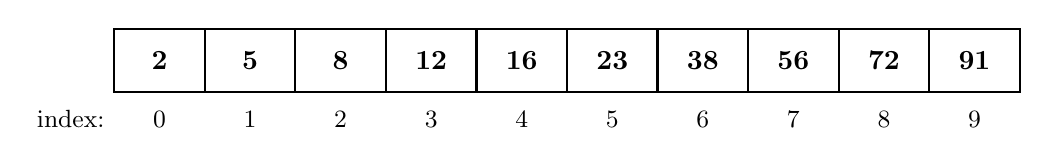
\begin{tikzpicture}[x=1.15cm]
  \foreach \v [count=\i from 0] in {2,5,8,12,16,23,38,56,72,91} {
    \draw[thick] (\i,0) rectangle ++(1,0.8);
    \node at (\i+0.5,0.4) {\textbf{\v}};
    \node[font=\small] at (\i+0.5,-0.35) {\i};
  }
  \node[font=\small,anchor=east] at (0,-0.35) {index:};
\end{tikzpicture}
\end{center}

\begin{center}
\renewcommand{\arraystretch}{1.6}
\begin{tabular}{|c|c|c|c|p{5.4cm}|}
\hline
\textbf{Step} & \textbf{low} & \textbf{high} & \textbf{middle} & \textbf{item at middle: too small, too big or found?}\\ \hline
1 & 0 & 9 & & \\ \hline
2 & & & & \\ \hline
3 & & & & \\ \hline
\end{tabular}
\end{center}
(a) Fill in the table. \quad (b) How many items would \textbf{linear} search (start at index 0) check
to find 23? \quad (c) A sorted list has 1000 items. About how many checks does binary search need
at most?
\answerlines{2}

\question{Sorting}{\textbf{Selection sort} finds the smallest item in the unsorted part and swaps it to
the front of the unsorted part. Write the list after each pass.}

\begin{tabular}{@{}ll@{}}
Start: & \texttt{[7, 3, 9, 1]}\\[6pt]
After pass 1: & \rule{5cm}{0.4pt}\\[10pt]
After pass 2: & \rule{5cm}{0.4pt}\\[10pt]
After pass 3: & \rule{5cm}{0.4pt}
\end{tabular}

Then: what does this print?
\begin{pycode}
def get_score(player):
    return player[1]

players = [("Mei", 40), ("Leo", 75), ("Ada", 60)]
best = sorted(players, key=get_score, reverse=True)
print(best[0][0])
\end{pycode}
\answerlines{1}

\question{Stacks and queues}{(a) What does this print?}
\begin{pycode}
from collections import deque

stack = []
stack.append("A")
stack.append("B")
stack.append("C")
print(stack.pop())

queue = deque()
queue.append("A")
queue.append("B")
queue.append("C")
print(queue.popleft())
\end{pycode}
(b) Stack or queue? Write \textbf{S} or \textbf{Q}: \quad an undo button \rule{1cm}{0.4pt}
\quad players waiting for their turn \rule{1cm}{0.4pt} \quad a pile of plates \rule{1cm}{0.4pt}
\answerlines{2}

\question{Explain}{Why is binary search usually faster than linear search? When can you
\textbf{not} use binary search?}
\answerlines{3}

\subsection{How am I doing halfway?}
\begin{icanrubric}
\ican{I can write a class with \texttt{\_\_init\_\_}, attributes and methods.}
\ican{I can make a child class that inherits and overrides a method.}
\ican{I can trace a binary search and explain why it is fast.}
\ican{I can explain how a sorting algorithm works.}
\ican{I can choose a stack or a queue for a job.}
\ican{I can commit my work with git and a helpful message.}
\end{icanrubric}

%% =====================================================================
\kcpart{Week 12}{Exit Assessment}{About 20 minutes. Read, predict, fix, design --- and explain.}
\setcounter{kcq}{0}
\namedateline

\subsection{Part A: Read and predict}

\question{Recursion}{What does \py|countdown(3)| print?}
\begin{pycode}
def countdown(n):
    if n == 0:
        print("Blast off!")
    else:
        print(n)
        countdown(n - 1)

countdown(3)
\end{pycode}
\answerlines{2}

\question{Recursion that returns}{What does this print? Show your thinking.}
\begin{pycode}
def total(n):
    if n == 1:
        return 1
    return n + total(n - 1)

print(total(4))
\end{pycode}
\answerlines{2}

\question{Grids}{(a) What does line 4 print? \quad (b) Which \texttt{[row][col]} holds
\texttt{"H"}? \quad (c) After line 5, what is in the top row?}
\begin{pycode}
grid = [["A", "B", "C"],
        ["D", "E", "F"],
        ["G", "H", "I"]]
print(grid[1][2], grid[2][0])
grid[0][1] = "#"
\end{pycode}
\answerlines{3}

\subsection{Part B: Find and fix}

\question{A recursion bug}{Sam's function should print a triangle of stars and stop, but it crashes
with \texttt{RecursionError}. Why? Rewrite it so it works.}
\begin{pycode}
def stars(n):
    print("*" * n)
    stars(n - 1)

stars(4)
\end{pycode}
\answerspace{3cm}

\question{A data bug}{Priya's \texttt{scores.csv} has a column \texttt{points}. Her program crashes
with \texttt{TypeError: unsupported operand type(s) for +: 'int' and 'str'}. Fix line 6. What
else could go wrong with real data, and how would you guard against it?}
\begin{pycode}
import csv

total = 0
with open("scores.csv", newline="") as file:
    for row in csv.DictReader(file):
        total = total + row["points"]
print(total)
\end{pycode}
\answerlines{3}

\subsection{Part C: How machines learn}

\question{Nearest neighbour}{An AI sorts monsters into \textbf{dragon} or \textbf{slime} using two
features. Distance = (difference in size) + (difference in spikes).}

\begin{center}
\renewcommand{\arraystretch}{1.4}
\begin{tabular}{|c|c|c|c|c|}
\hline
\textbf{Example} & \textbf{size (1--10)} & \textbf{spikes (0--5)} & \textbf{label} & \textbf{distance to mystery}\\ \hline
A & 9 & 4 & dragon & \\ \hline
B & 8 & 5 & dragon & \\ \hline
C & 2 & 0 & slime & \\ \hline
D & 3 & 1 & slime & \\ \hline
\textbf{Mystery} & \textbf{4} & \textbf{1} & \textbf{?} & --- \\ \hline
\end{tabular}
\end{center}
(a) Fill in the distances. \quad (b) What does the AI predict for the mystery monster, and why?
\answerlines{2}

\question{When AI gets it wrong}{A fruit-sorting AI was trained only on photos of
\textbf{red} apples. (a) What might happen when it sees a green apple? (b) What is this problem
called? (c) How would you fix it?}
\answerlines{3}

\question{Using AI safely}{(a) Name two things you should never type into an AI chatbot.
(b) A Markov text generator writes funny, strange sentences. Why does it not really
\enquote{understand} what it writes?}
\answerlines{3}

\subsection{Part D: Design and explain}

\question{Design a game}{You are planning a \textbf{treasure-map game}: a 10 by 10 map with walls, a
player, treasure and a monster that always takes the shortest way to the player.
(a) Which data structure would you use for the map? (b) Which algorithm should the monster use?
Which data structure does that algorithm need? (c) Name two classes, with one attribute and one
method each. Would one inherit from the other, or use composition? Why?}
\answerspace{5.5cm}

\question{Your design decision}{Describe one design decision in your own final project: what you
chose, one other way you could have done it, and why your way is better (or what you would change
now).}
\answerspace{4cm}

\subsection{How far have I come in Level 3?}
\begin{icanrubric}
\ican{I can design a program with classes, inheritance and composition.}
\ican{I can write a recursive function with a base case.}
\ican{I can use a 2D grid (\texttt{grid[row][col]}).}
\ican{I can clean data from a CSV file and chart it.}
\ican{I can explain how a nearest-neighbour AI makes a prediction, and how it can be unfair.}
\ican{I can track my project with git and test it with pytest.}
\ican{I can explain why I designed my program the way I did.}
\end{icanrubric}

\begin{reflection}[Looking back]
What are you most proud of from Level 3? What do you want to build next?
\answerlines{3}
\end{reflection}

\end{document}
